\chapter*{Guía de Reflexión y Meditación}
\addcontentsline{toc}{chapter}{Guía de Reflexión y Meditación}
\markboth{Guía de Reflexión y Meditación}{Guía de Reflexión y Meditación}
\vspace{0.6cm}
\begin{center}
\nopagebreak
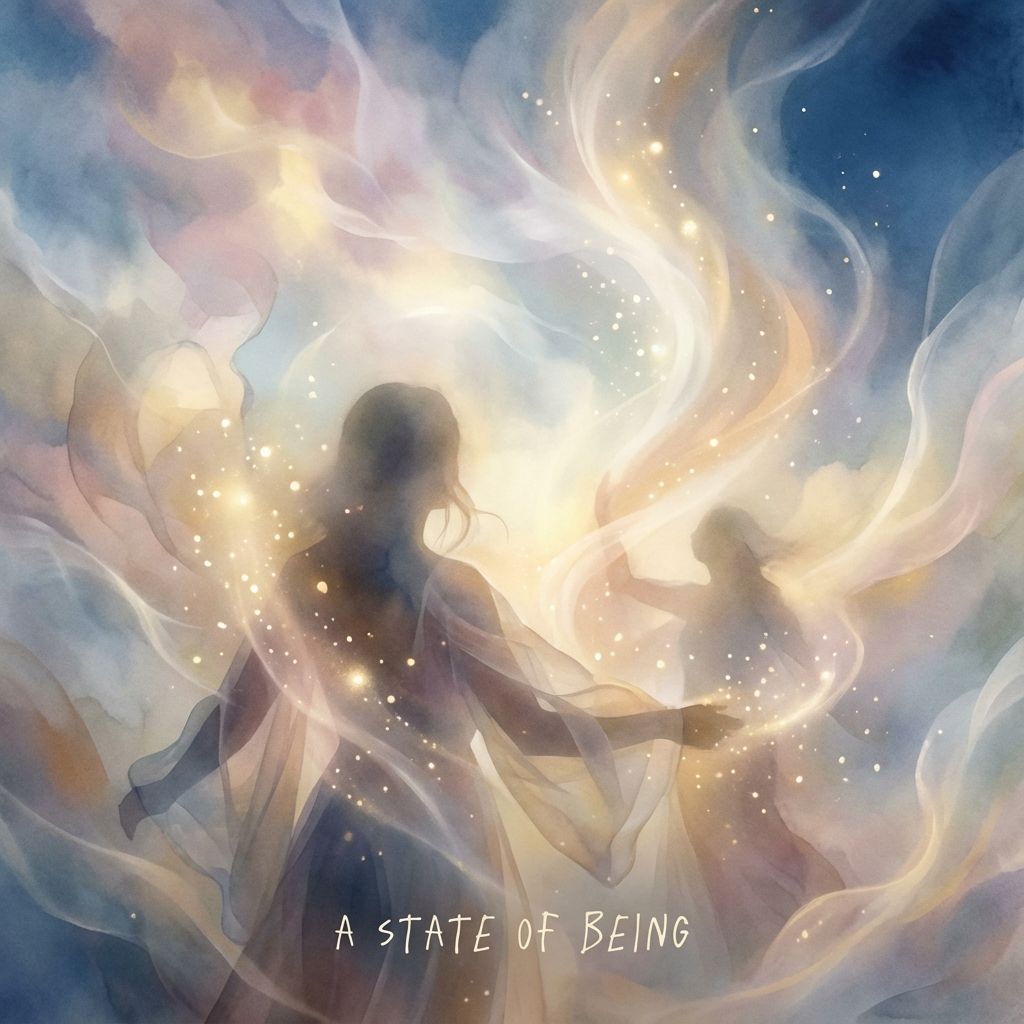
\includegraphics[width=0.75\textwidth,cfbox=gray!60 0.6pt 4pt]{heaven_state.png}\\
\vspace{4pt}
{\small\itshape El templo interior: guía de presencia, silencio y coherencia cuántica.}
\end{center}

\vspace{0.6cm}
Para transformar los conceptos del libro en una experiencia viva en tu día a día, te sugerimos esta pequeña práctica de alineación cuántica en tres pasos:


\vspace{0.4cm}
\begin{center}
\rule{0.35\textwidth}{0.4pt}
\end{center}
\vspace{0.4cm}


\subsection*{1. La Pausa del Observador (Silencio Consciente)}
\noindent\textbullet~~Encuentra un momento de tranquilidad al comenzar o finalizar el día.\\

\noindent\textbullet~~Cierra los ojos y realiza tres respiraciones lentas y profundas, inhalando calma y exhalando cualquier preocupación.\\

\noindent\textbullet~~Conviértete en el «observador» imparcial de tus pensamientos sin juzgarlos. Recuerda que tú no eres el ruido mental; eres el espacio consciente en el que el ruido ocurre.\\



\vspace{0.4cm}
\begin{center}
\rule{0.35\textwidth}{0.4pt}
\end{center}
\vspace{0.4cm}


\subsection*{2. El Reajuste de Frecuencia (El Aliento de Abwoon)}
\noindent\textbullet~~Lleva tu atención al centro del pecho (la coherencia cardíaca).\\

\noindent\textbullet~~Evoca un recuerdo o sentimiento genuino de gratitud, aprecio o amor sincero.\\

\noindent\textbullet~~Siente cómo esa emoción eleva instantáneamente tu estado vibracional y disuelve las cargas de miedo o pesadez.\\



\vspace{0.4cm}
\begin{center}
\rule{0.35\textwidth}{0.4pt}
\end{center}
\vspace{0.4cm}


\subsection*{3. Preguntas para tu Cuaderno Interior}
Dedica unos minutos a reflexionar o escribir sobre estas preguntas:
\noindent\textbf{1.}~~\textit{¿En qué situaciones cotidianas siento que mi frecuencia vibratoria disminuye y cómo puedo elegir responder con amor?}\\

\noindent\textbf{2.}~~\textit{¿Existe algún lazo del pasado que esté listo para disolver mediante el perdón consciente hoy?}\\

\noindent\textbf{3.}~~\textit{¿Cómo puedo ser un reflejo vivo de la Luz y la Presencia para las personas que me rodean?}\\



\vspace{0.4cm}
\begin{center}
\rule{0.35\textwidth}{0.4pt}
\end{center}
\vspace{0.4cm}




\begin{quote}
\itshape \textit{«La paz no es la ausencia de movimiento en el mundo exterior, sino la presencia inquebrantable de la Luz en tu interior.»}
\end{quote}